\chapter{初等数论：质数、同余与整数的机关}

\section{拆不开的班：从一次排队说起}

学校开运动会，体育老师要把初二年级的同学排成若干行，要求每行人数一样多，不许有落单的。六年级三个班各报了自己的人数：甲班 $48$ 人，乙班 $45$ 人，丙班 $47$ 人。

甲班很快搞定了：$48$ 人可以排成 $6$ 行 $8$ 列，也可以排成 $4$ 行 $12$ 列，花样多得很。乙班也不愁：$45$ 人可以排成 $5$ 行 $9$ 列。轮到丙班，大家试了半天：每行 $2$ 人？剩一个。每行 $3$ 人？剩一个。每行 $4$ 人、$5$ 人、$6$ 人……全都剩一个。$47$ 这个数像一块摔不碎的石头，怎么都拆不成两个比它小的整数相乘。

先凭直觉猜一猜：这样的“石头数”是很少见的怪胎，还是其实满地都是？它们有没有一个尽头——比如说，比某个数更大的整数全都能被拆开？这个问题听起来像小孩子数数时随口一问，却难住过历史上最聪明的头脑。这一章我们就从这块“石头”出发，看看整数内部藏着哪些机关。

\section{第一次尝试：筛子和误会}

遇到$47$拆不开，最朴素的办法是把可能的因数挨个试一遍。$2$ 不行（$47$ 是奇数），$3$ 不行（$4+7=11$ 不是 $3$ 的倍数），$5$ 不行（末位不是 $0$ 或 $5$），$7$ 呢？$7\times 6=42$，$7\times 7=49$，也不行。试到这里其实可以停了——为什么？因为 $7\times 7=49$ 已经超过 $47$ 了。如果 $47$ 能写成两个都大于 $1$ 的整数相乘，其中至少有一个不超过它的平方根 $\sqrt{47}\approx 6.9$。试到 $6$ 就够了，不必试到 $46$。这是本章第一个“机关”：检验一个数能不能拆开，只需要检查到它的平方根。

顺着这个思路，有人提出一个大胆的猜想：“拆不开的数就是奇数。”听起来有道理，偶数不都能拆出 $2$ 吗？但立刻有人反驳：$9$ 是奇数，却等于 $3\times 3$；$15$、$21$、$25$ 也都拆得开。反过来，$2$ 是偶数，却拆不开。看来“奇偶”和“能不能拆开”是两回事。

\begin{fanli}
“奇数都是拆不开的数”——错误。$9=3\times3$、$15=3\times5$、$21=3\times7$ 都是奇数，却都能拆成更小的整数相乘。判断一个数能否拆开，唯一可靠的办法是检查到平方根为止的所有可能因数，而不是看它的末位或奇偶。
\end{fanli}

两千多年前，古希腊的数学家想出了一个系统性的办法，后人称之为“筛法”：把 $2$ 到 $100$ 的数全写出来，圈起 $2$，划掉所有 $2$ 的倍数；找到下一个没被划掉的数 $3$，圈起来，划掉所有 $3$ 的倍数；再找到 $5$、$7$……凡是被划掉的，都是能被更小的数整除的“合成品”；最后剩下的，就是那些摔不碎的石头。这个方法笨，但诚实——它保证一个不漏。

这里还有一个容易错过的省力之处：划到 $7$ 的倍数时就可以收工了。因为按平方根界限，$100$ 以内的任何合数必有一个不超过 $\sqrt{100}=10$ 的质因数，也就是说它早就在划 $2,3,5,7$ 的倍数时被干掉了。四轮之后幸存下来的，一定全是拆不开的数。筛完 $100$ 以内的数，剩下的是这张清单：

\begin{center}
\begin{tabular}{rrrrr}
\toprule
$2$ & $3$ & $5$ & $7$ & $11$\\
$13$ & $17$ & $19$ & $23$ & $29$\\
$31$ & $37$ & $41$ & $43$ & $47$\\
$53$ & $59$ & $61$ & $67$ & $71$\\
$73$ & $79$ & $83$ & $89$ & $97$\\
\bottomrule
\end{tabular}
\end{center}

数一数，共 $25$ 个。盯着这张表看一会儿，你会生出许多问题：为什么除了 $2$ 全是奇数？为什么越往后间隔好像越大？为什么有的紧紧挨着（$41$ 和 $43$），有的却隔得很远？这些问题我们很快就会一一捡起来——其中有的已经有答案，有的至今没有。

\section{发明概念：质数是整数的“原子”}

被筛子剩下的数值得一个正式的名字。

\begin{dingyi}[质数与合数]
大于 $1$ 的整数，如果除了 $1$ 和它本身之外没有别的正因数，就称为\emph{质数}（也叫素数）；否则称为\emph{合数}。数 $1$ 既不是质数也不是合数。
\end{dingyi}

这里最容易被问倒的是：“凭什么把 $1$ 开除出质数队伍？$1$ 不也只能被 $1$ 和自己整除吗？”这是一个真正的好问题，答案不在定义本身，而在后面要讲的一个定理：数学家希望“每个整数的拆法唯一”，如果让 $1$ 混进质数里，$6$ 就能写成 $2\times3$、$1\times2\times3$、$1\times1\times2\times3$……拆法就不唯一了。把 $1$ 请出去，是为了让整数的乘法世界有一条干净的基本定律。定义不是天经地义的，而是为了让定理说得漂亮而精心设计的。

\begin{shuyu}{质数}
\textbf{直观解释}：整数世界里摔不碎的“原子”，只能由 $1$ 和它自己搭出来，拆不成更小的整数乘积。

\textbf{正式定义}：大于 $1$ 且正因数只有 $1$ 与自身的整数。

\textbf{一个例子}：$47$ 是质数，因为 $2,3,5$ 都整除不了它，而 $7>\sqrt{47}$，检验可以到此为止。
\end{shuyu}

化学家发现世间万物由一百多种原子构成，数论学家则发现：每个大于 $1$ 的整数都由质数“搭”出来。$48=2\times2\times2\times2\times3$，$45=3\times3\times5$，而 $47$ 本身就是一块原子。更惊人的是，搭法只有一种。

\begin{dingli}[算术基本定理]
每个大于 $1$ 的整数都可以唯一地分解为质数的乘积，若不计较这些质数的书写顺序，分解方式是唯一的。
\end{dingli}

先看分解的“存在性”，它几乎是一棵树的自然生长：任取一个合数，把它拆成两个更小的数；拆出来的数如果还是合数，就继续拆。每拆一次，数都严格变小，而整数不会无穷变小下去，所以这个过程必然停在某处——停下来的那些数拆不动了，正是质数。图里画出了 $360$ 的一棵分解树。

\begin{center}
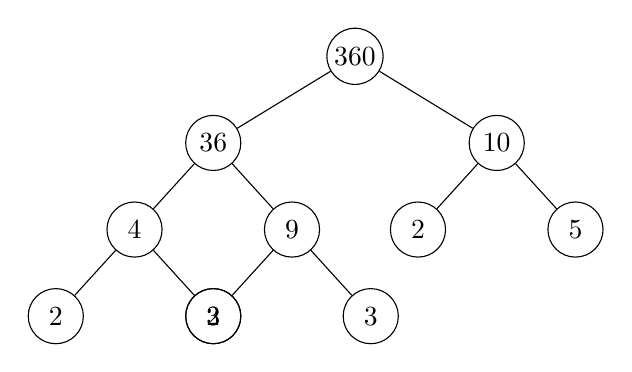
\begin{tikzpicture}[level distance=11mm,
  level 1/.style={sibling distance=36mm},
  level 2/.style={sibling distance=20mm},
  every node/.style={circle,draw,inner sep=1.5pt,minimum size=7mm}]
\node {360}
  child { node {36}
    child { node {4}
      child { node {2} }
      child { node {2} } }
    child { node {9}
      child { node {3} }
      child { node {3} } } }
  child { node {10}
    child { node {2} }
    child { node {5} } };
\end{tikzpicture}
\end{center}

把所有“树叶”乘起来：$360=2^3\times 3^2\times 5$。换一条路拆（比如先拆成 $12\times 30$），叶子还是同一批质数，只是碰见的顺序不同。

“唯一性”则要费一点脑筋。凭什么不能存在两套完全不同的质数，乘出来恰好是同一个数？关键在于下面这个引理：

\begin{tuilun}[质数整除引理]
若质数 $p$ 整除乘积 $ab$，则 $p$ 整除 $a$ 或整除 $b$。
\end{tuilun}

这个引理对合数是假的（$6$ 整除 $3\times 4=12$，但 $6$ 既不整除 $3$ 也不整除 $4$），它的证明要用到下一节的最大公因数，我们先把证明思路存在那里。有了引理，唯一性就好办了：假如某个数有两套质数分解，把两套写法都列出来，左边第一个质数整除右边的乘积，由引理它必然整除右边某一个质数——而质数只能被自己和 $1$ 整除，所以它们其实是同一个质数。两边同时约掉它，对剩下的部分重复同样的话，最后两边的质数必然一模一样。直觉上“拆法只有一种”是对的，而且是被严格证明了的。

\section{辗转相除：一台两千岁的机器}

现在来补那个引理欠下的工具。给定两个整数，比如 $252$ 和 $105$，它们公共的因数里最大的是谁？这个数叫最大公因数。笨办法是把两个数各自的所有因数列出来再找交集，但有个快得惊人的老办法，写在两千多年前的古希腊数学书里，今天还在你手机的芯片里跑着。

\begin{dingyi}[最大公因数]
整数 $a$、$b$（不全为 $0$）的公共因数中最大的一个，记作 $\gcd(a,b)$。若 $\gcd(a,b)=1$，称 $a$ 与 $b$ \emph{互质}。
\end{dingyi}

\begin{shiyan}
拿一张纸算 $\gcd(252,105)$。第一步：$252$ 除以 $105$，商 $2$ 余 $42$，写下 $252=2\times105+42$。第二步：拿刚才的除数 $105$ 除以刚才的余数 $42$，$105=2\times42+21$。第三步：$42$ 除以 $21$，$42=2\times21+0$，余数为 $0$，停。最后那个不为零的余数 $21$ 就是答案：$\gcd(252,105)=21$。全程三次除法，不需要知道 $252$ 或 $105$ 的任何因数。
\end{shiyan}

这个办法叫欧几里得算法（辗转相除法）。它为什么对？核心是一句话：若 $a=bq+r$，那么 $a$ 和 $b$ 的公共因数，与 $b$ 和 $r$ 的公共因数，是完全相同的一批数。道理在于：凡是 $b$ 和 $r$ 的公因数，必然整除 $bq+r=a$；反过来，凡是 $a$ 和 $b$ 的公因数，必然整除 $a-bq=r$。公因数队伍原班不动，最大者当然也相同，于是
\[
\gcd(a,b)=\gcd(b,r).
\]
而右边的数越来越小，余数一路减小又不可能小于 $0$，若干步后必然余 $0$，此时较小的那个数就是答案。它不依赖质因数分解——这恰恰是它强大的原因，因为分解大整数恰恰是很难的（这一点后面还会救密码学一命）。

这个算法有一个几何版本，美得像一幅画：给一个 $252\times 105$ 的长方形，用最大的正方形去铺它。先铺下两个 $105\times 105$ 的正方形，剩下 $42\times 105$ 的长条；再用 $42\times 42$ 的正方形铺这个长条，铺两个剩 $42\times 21$；最后用 $21\times 21$ 正好铺满。最后那种正方形恰好铺满不剩边角，它的边长就是最大公因数。铺不下去的余量越来越小，正如余数越来越小。

还有一个副产品：把辗转相除的算式倒着读回去，能把最大公因数写成原来两数的“整系数组合”。在上面的例子里：
\[
21=105-2\times42=105-2\times(252-2\times105)=5\times105-2\times252.
\]
一般结论是：总存在整数 $x,y$ 使 $\gcd(a,b)=ax+by$。别小看这一行式子，上一节的“质数整除引理”就靠它：设质数 $p$ 整除 $ab$ 却不整除 $a$，那么 $\gcd(p,a)=1$（$p$ 的正因数只有 $1$ 和 $p$），于是有整数 $x,y$ 使 $px+ay=1$。两边乘 $b$ 得 $pbx+aby=b$。左边第一项显然被 $p$ 整除，第二项里的 $ab$ 按假设也被 $p$ 整除，所以 $b$ 被 $p$ 整除。引理得证，算术基本定理的最后一颗螺丝拧紧了。

最大公因数还有一个日常用途：约分。分数 $\frac{252}{105}$ 要约到最简，只需分子分母同除以 $\gcd(252,105)=21$，一步得到 $\frac{12}{5}$，不必试探性地反复约。与它搭档的是最小公倍数：两个整数的最小公倍数乘以最大公因数，恰好等于两数之积，即 $\mathrm{lcm}(a,b)\cdot\gcd(a,b)=ab$。所以 $252$ 与 $105$ 的最小公倍数是 $252\times105\div21=1260$。一个例子让你看到它在哪出现：两盏霓虹灯分别每 $252$ 秒和每 $105$ 秒闪一次，从同闪到下一次同闪，间隔正是 $1260$ 秒——所有“重逢”问题（齿轮重新对齐、行星再次连珠、公交两车同时到站）背后都是这一个数。

\section{奇偶、不变量与同余：换一种眼光看整数}

分解关心的是乘法结构。现在换一个角度：不关心一个数“是谁”，只关心它“属于哪一类”。最简单的分类是奇与偶——被 $2$ 除余 $1$ 还是余 $0$。可别嫌它简单，它是一件威力巨大的武器，学名叫\emph{不变量}。

经典的一幕：一个 $8\times8$ 的棋盘，挖掉对角上的两个格子，能用 $31$ 张 $1\times2$ 的多米诺骨牌正好铺满吗？你可以试一个下午，每次都差一点点。数学家不试，他只看颜色：每张骨牌无论横放竖放，必然盖住一黑一白两个格子，所以铺得满的图形黑白格子必须一样多。而被挖掉的两个对角格子是同色的，剩下的棋盘上黑格比白格多两个（或少两个）。$31$ 张骨牌盖 $31$ 黑 $31$ 白，永远对不上 $30$ 与 $32$。一次尝试都不用，答案就是“不可能”。奇偶性在铺砖过程中保持不变——正是这个“不变”宣判了死刑。

奇偶是“除以 $2$ 的余数”。把这个想法推广到除以任何数，就得到数论里最好用的工具之一。

\begin{dingyi}[同余]
设 $m$ 是正整数。若整数 $a$ 与 $b$ 被 $m$ 除所得的余数相同（等价地，$m$ 整除 $a-b$），就说 $a$ 与 $b$ \emph{模 $m$ 同余}，记作
\[
a\equiv b\pmod{m}.
\]
\end{dingyi}

\begin{shuyu}{同余}
\textbf{直观解释}：钟面上的算术。现在下午 $3$ 点，过 $14$ 小时是几点？$3+14=17$，$17\equiv5\pmod{12}$，即凌晨 $5$ 点。钟面上 $17$ 和 $5$ 是同一个位置。

\textbf{正式定义}：$a\equiv b\pmod{m}$ 当且仅当 $m$ 整除 $a-b$。

\textbf{一个例子}：$100\equiv2\pmod{7}$，所以从今天起过 $100$ 天，星期几只取决于 $2$——往后数两天即可。
\end{shuyu}

同余的妙处在于它像等号一样好用：同余式两边可以同时加、减、乘同一个整数。于是处理巨大的数时，可以随时把它换成模 $m$ 意义下的小替身。想算 $7^{100}$ 的个位数？个位数就是模 $10$ 的余数。$7^2=49\equiv9\pmod{10}$，$7^4\equiv9^2=81\equiv1\pmod{10}$，于是
\[
7^{100}=(7^4)^{25}\equiv 1^{25}=1\pmod{10}.
\]
个位数是 $1$。我们从没算出 $7^{100}$ 这个有八十多位的庞然大物，却知道了它的末位——这就是“只看类别”的力量。

同余还能解释一些你早就背过、却未必想过为什么的口诀。比如：“一个数能被 $3$ 整除，当且仅当它的各位数字之和能被 $3$ 整除。”为什么数字会这么听话？秘密在于 $10\equiv1\pmod3$（同样 $10\equiv1\pmod9$）。于是 $10$ 的任何次幂模 $3$ 都是 $1$，一个四位数展开后：
\[
\overline{abcd}=1000a+100b+10c+d\equiv a+b+c+d\pmod{3}.
\]
换句话说，十进制写法本身就把一个数和它的数字和绑在了同一“类”里。拿 $123\,456$ 试试：数字和为 $1+2+3+4+5+6=21$，是 $3$ 的倍数但不是 $9$ 的倍数，所以 $123\,456$ 能被 $3$ 整除而不能被 $9$ 整除——不必真的做除法。老式会计还有一个叫“弃九法”的验算招术：检查乘法 $47\times 62=2914$ 是否可信，就把 $47$、$62$、$2914$ 各自的数字和反复加到一个数字为止（$47\to11\to2$，$62\to8$，$2914\to16\to7$），看 $2\times8=16\to7$ 是否与积的数字根吻合。吻合不一定对，不吻合一定错——这是一种古老的“纠错码”，原理正是模 $9$ 同余。

把同余推到精致处，会碰到一颗小宝石，由十七世纪的法国数学家费马发现（他常以在书页空白处写下惊人断言而闻名）：

\begin{dingli}[费马小定理]
设 $p$ 是质数，整数 $a$ 不是 $p$ 的倍数，则
\[
a^{p-1}\equiv1\pmod{p}.
\]
\end{dingli}

\begin{proof}
考察 $p-1$ 个数 $a,2a,3a,\dots,(p-1)a$ 被 $p$ 除的余数。先说它们两两不同余：若 $ia\equiv ja\pmod p$（不妨 $i>j$），则 $p$ 整除 $(i-j)a$；由质数整除引理，$p$ 整除 $i-j$ 或整除 $a$，但 $a$ 不是 $p$ 的倍数，且 $0<i-j<p$，都不可能。所以这 $p-1$ 个余数互不相同，又都不为 $0$（否则 $p$ 整除某个 $ia$，同样矛盾），恰好是 $1,2,\dots,p-1$ 的一个重排。把这 $p-1$ 个数全部乘起来，一方面
\[
a\cdot2a\cdots(p-1)a=a^{p-1}\cdot(p-1)!\,,
\]
另一方面，模 $p$ 意义下这批余数乘起来就是 $1\cdot2\cdots(p-1)=(p-1)!$。两边同余：
\[
a^{p-1}\cdot(p-1)!\equiv(p-1)!\pmod p.
\]
$(p-1)!$ 与 $p$ 互质，可以约去，即得 $a^{p-1}\equiv1\pmod p$。
\end{proof}

配一个数值例子：取 $p=11$，$a=2$。$2^5=32\equiv-1\pmod{11}$，所以 $2^{10}\equiv(-1)^2=1\pmod{11}$。定理预言的事分毫不差。这个定理看上去像纯游戏，三百年后却成了银行系统的基石——谜底在下一节揭晓。

\begin{zhu}
定理反过来却不成立：存在合数 $n$，也能让某些 $a$ 满足 $a^{n-1}\equiv1\pmod n$，例如 $341=11\times31$ 就能“骗过”以 $2$ 为底的检验。这类数叫伪质数。所以费马小定理可以铁口直断“不是质数”（同余不成立时），却只能在概率意义上说“像是质数”——现代计算机检验大质数，正是从这条缝里发展出的一整套技术。
\end{zhu}

\section{质数用不完：一个两千多年前的证明}

回到开头的疑问：丙班那种“石头数”，会不会到某个地方就没有了？会不会分解超大整数时，最终只遇到质数库里有限的存货？古希腊人给出了回答，而且这个回答被公认为数学史上最漂亮的证明之一。

\begin{dingli}[质数有无穷多个]
不存在“最大的质数”：任给一个质数，总能找到比它更大的质数。
\end{dingli}

\begin{proof}
用反证法。假设质数只有有限多个，把它们全部列出来：$p_1,p_2,\dots,p_n$。构造一个新整数
\[
N=p_1\,p_2\,\cdots\,p_n+1,
\]
即“所有质数乘起来再加 $1$”。$N$ 大于 $1$，由算术基本定理，$N$ 必能被某个质数整除。这个质数是谁？不可能是 $p_1$：$N$ 除以 $p_1$ 余 $1$。也不可能是 $p_2,p_3,\dots,p_n$ 中的任何一个——$N$ 除以它们每一个都余 $1$。所以存在一个不在清单上的质数整除 $N$，与“清单已穷尽所有质数”矛盾。假设错误，质数不可能只有有限个。
\end{proof}

请留意这个证明的结构：它没有告诉你下一个质数在哪，只是证明了“清单永远列不完”。这种“假设反面成立，推出自相矛盾”的反证法，是数学家工具箱里最锋利的工具之一。另外注意一个细节：$N$ 本身不一定是质数。比如 $2\times3\times5\times7\times11\times13+1=30031$，它等于 $59\times509$，是合数——但它确实被清单之外的新质数 $59$ 和 $509$ 整除，证明的关键只在这里，不在 $N$ 是否本身是质数。

顺便一提，质数虽无穷，分布却越来越稀疏，而且极不规律。在 $1$ 到 $100$ 之间，质数有 $25$ 个，占了四分之一；到 $1000$ 附近，每十个数里大约只剩一个半质数；数越大，质数越罕见——这符合直觉，数越大，能成为它因数的“候选”越多，想保持拆不开就越难。数学家甚至证明了：想找出连着一千个整数的“质数沙漠”也可以，因为 $1001!+2,1001!+3,\dots,1001!+1001$ 分别被 $2,3,\dots,1001$ 整除，整整一千个连续的合数。

可另一方面，质数又拒绝彻底疏远。像 $3$ 与 $5$、$17$ 与 $19$、$101$ 与 $103$ 这样只差 $2$ 的“孪生质数”，目前已知的最大一对有几十万位。它们是否也有无穷多对？这就是著名的孪生质数\emph{猜想}——至今既没被证明也没被推翻，人类只证明了“相差不超过某个固定上限的质数对有无穷多”这样的近似版本。越稀、越乱，却似乎永不彻底孤单：质数的分布是数学中最大的悬案之一，我们把它放进“继续攀登”里。

\section{换一个视角：这些机关如何锁住现代世界}

数论曾被称为“数学的皇后”，以纯粹、无用而自豪。二十世纪下半叶，情况戏剧性地反转：今天每次网购、每条加密消息、每张刷过的公交卡，都在调用这一章的机关。

\textbf{第一道机关：纠错码。} 每本书封底的国际标准书号（ISBN）由一串数字组成，最后一位是“校验位”，由前面的数字按模运算算出。一种经典方案是：前九位 $a_1,a_2,\dots,a_9$ 分别乘以权重 $10,9,\dots,2$ 后求和，再选校验位 $x$ 使总和被 $11$ 整除：
\[
10a_1+9a_2+\cdots+2a_9+x\equiv0\pmod{11}.
\]
假设前九位是 $9,7,8,7,0,4,0,0,3$，加权和为
\[
90+63+64+49+0+20+0+0+6=292,
\]
而 $292=11\times26+6$，所以取 $x\equiv-6\equiv5\pmod{11}$，校验位是 $5$。它的用处在于：如果录入时某一位抄错了，加权和就不再被 $11$ 整除，系统立刻报警；甚至两位数字对调也能被发现。为什么模 $11$ 而不是模 $10$？诀窍正在于 $11$ 是质数：相邻两位对调时，加权和的改变量是权重之差乘以数字之差，即 $\pm(a_i-a_{i+1})$；只要两位数字不同，这个改变量就含一个介于 $\pm1$ 与 $\pm9$ 之间的因子，而质数 $11$ 不可能整除这样的小整数，于是错误必然暴露。若模 $10$，数字差为 $5$ 的对调就会被漏检。同样的心思藏在银行卡号、快递单号和二维码里：故意多存一点“按规则可预测”的信息，让错误无处藏身。二维码走得更远，它存的不只一位校验，而是成块的冗余信息，所以图案被污渍盖住一角、甚至被印上一个小商标，手机照样读得出来——那是更强壮的纠错码，背后仍是同一套模运算的算术。

\textbf{第二道机关：公开密钥密码。} 传统密码像一把挂锁，锁和开用同一把钥匙，传递钥匙本身就成了破绽。二十世纪七十年代，数学家们提出一个看似异想天开的方案：把锁公开送人，钥匙自己留着——任何人都能锁上盒子寄给你，但只有你能开。实现它的正是质数、同余和费马小定理。一个简化模型如下（真实系统用的是几百位的大数，原理相同）：

\begin{enumerate}
  \item 你秘密选两个质数 $p=3$、$q=11$，公开它们的乘积 $N=33$，但 $p$、$q$ 本身保密。
  \item 由费马小定理的思想可以推知，取适当的“公开指数” $e=3$ 和“秘密指数” $d=7$（它们满足 $ed\equiv1\pmod{(p-1)(q-1)}$，即 $21\equiv1\pmod{20}$），则对任何信息 $m$ 都有 $(m^e)^d\equiv m\pmod N$。
  \item 朋友要寄给你数字 $m=4$，用公开的 $(N,e)$ 加密：$4^3=64\equiv31\pmod{33}$，把 $31$ 寄出。
  \item 你收到 $31$，用秘密的 $d$ 解密：$31^7\pmod{33}$。手算验证：$31\equiv-2\pmod{33}$，$(-2)^7=-128$，而 $-128\equiv4\pmod{33}$。信息 $4$ 原样归来。
\end{enumerate}

窃听者看到的是 $N=33$、$e=3$ 和密文 $31$。要推回 $d$，本质上需要知道 $(p-1)(q-1)$，也就是需要把 $N$ 分解回 $3\times11$。$33$ 当然谁都会分，但把 $N$ 换成两个三百位质数的乘积，人类现有最快的计算机算上宇宙年龄也分解不完。加密容易、分解难——安全的根基不是算法保密，而是分解大整数这件事本身的艰难。当年“最无用”的费马小定理，如今每天保护着天文数字的资金流动。

\begin{lianjie}
这一章串起了一条出人意料的因果链：欧几里得两千多年前的辗转相除，支撑了算术基本定理的唯一性；费马十七世纪的一则小定理，配上“分解大整数很难”这个至今无人攻破的经验事实，变成了现代互联网的安全锁。数学里“没用”和“有用”之间的距离，有时需要几百年才能走完——这也是判断一个理论价值时该有的耐心。
\end{lianjie}

\begin{toolbox}
本章新增的数论工具：
\begin{itemize}
  \item \textbf{平方根界限}：检验 $n$ 是否为质数，只需试除到 $\sqrt{n}$。
  \item \textbf{质因数分解}：每个整数唯一地写成质数幂的乘积（算术基本定理）。
  \item \textbf{辗转相除}：$\gcd(a,b)=\gcd(b,r)$，其中 $a=bq+r$；倒推还能写出 $\gcd(a,b)=ax+by$。
  \item \textbf{不变量}：找一个在过程中保持不变的量（如奇偶性、黑白格数之差），用它判定“不可能”。
  \item \textbf{同余}：$a\equiv b\pmod{m}$，大数随时换成小替身，加减乘保持同余。
  \item \textbf{反证法}：假设结论不成立，推出矛盾（质数无穷多的证明是范本）。
\end{itemize}
\end{toolbox}

\begin{pandeng}
想继续往上爬，可以查这些关键词：\textbf{素数定理}（不超过 $x$ 的质数约有 $x/\ln x$ 个，质数虽无穷却越来越稀）；\textbf{哥德巴赫猜想}（每个大于 $2$ 的偶数都是两个质数之和，至今未证）；\textbf{黎曼猜想}（质数分布的终极密码，悬赏百万美元）；\textbf{二次剩余与互反律}；\textbf{中国剩余定理}（“韩信点兵”问题的完整理论）；\textbf{椭圆曲线密码}（RSA 之后的新一代公钥体系）。
\end{pandeng}

\section*{思考题}

\textbf{观察题}
\begin{sikao}
  \item 写出 $2$ 到 $50$ 之间所有的孪生质数对（相差为 $2$ 的质数对）。数一数有几对。提示：先用筛法列出 $50$ 以内的全部质数，再找相邻差为 $2$ 的对子；注意 $(3,5)$、$(5,7)$、$(11,13)$ 这样的形状。
  \item 观察 $n^2+n+41$ 在 $n=0,1,2,3,4$ 时的值，它们似乎都是质数。提示：别急着下结论，继续代几个更大的 $n$ 试试，特别留意某个“显然特殊”的取值。
\end{sikao}

\textbf{证明题}
\begin{sikao}
  \item 证明：除 $2,3$ 之外，每个质数都具有 $6k+1$ 或 $6k+5$ 的形状（$k$ 为整数）。提示：任何整数被 $6$ 除的余数只有六种，逐个检查 $6k$、$6k+2$、$6k+3$、$6k+4$ 为什么是合数。
  \item 证明：若 $a\equiv b\pmod{m}$ 且 $c\equiv d\pmod{m}$，则 $ac\equiv bd\pmod{m}$。提示：从定义出发，把 $a=b+sm$、$c=d+tm$ 代入乘积展开，看哪些项含因数 $m$。
\end{sikao}

\textbf{挑战题}
\begin{sikao}
  \item 求 $2^{2025}$ 被 $7$ 除的余数。提示：先算 $2^1,2^2,2^3,\dots$ 模 $7$ 的余数，观察循环规律（或者用费马小定理，$7$ 是质数）。
  \item 在公开密钥的例子里，我们用了 $p=3$、$q=11$、$e=3$、$d=7$。请你用 $p=5$、$q=7$ 自己搭建一套：算出 $N$ 和 $(p-1)(q-1)$，选一个与 $(p-1)(q-1)$ 互质的 $e$，再找出满足 $ed\equiv1\pmod{(p-1)(q-1)}$ 的 $d$（倒用辗转相除），最后加密并解密一个你自己选的信息，验证能还原。提示：$e$ 可以取 $5$；找 $d$ 就是解同余方程 $5d\equiv1\pmod{24}$。
\end{sikao}

\section*{通往下一章的门}

这一章里，我们反复在做同一件朴素的事：\emph{数}。筛法是在数质数，棋盘问题是在数黑白格，费马小定理的证明是把 $p-1$ 个数“数了两遍”——先按原样乘，再按余数重排乘，两种数法给出同一个结果，定理就从等号里掉了出来。最后这个手法尤其值得回味：换一种方式清点同一批对象，竟能推出根本不显然的结论。

可一旦认真去“数”，问题立刻变多：质数定理说质数大约有 $x/\ln x$ 个，“大约”到底怎么数出来的？一副扑克牌有多少种洗牌结果？$8\times8$ 棋盘上放 $8$ 个互不攻击的皇后，有几种放法？摩尔斯电码里，由五个点划组成的不同信号有多少种？这些问题里，对象不再是孤零零的整数，而是成堆的排列、选取、摆放方式——它们是离散的、一个一个的。怎样系统地清点它们而不重复、不遗漏？这正是下一章的主角：组合与离散结构。我们会看到，“数清楚”本身是一门有定理、有技巧、有陷阱的学问，而本章的整数机关——奇偶、同余、互质——会在那里反复登场。
